\documentclass[titlepage]{octavo}
\usepackage[lmargin=1.8cm]{geometry}
\usepackage[utf8]{inputenc}
\usepackage{lettrine}
\usepackage{tgchorus}
\usepackage[T1]{fontenc}
\usepackage{niceframe}
\usepackage{parselines}
\usepackage{graphicx}
\usepackage{xcolor}
\definecolorseries{verso}{rgb}{last}{blue!40!black}{magenta!40!black}
\resetcolorseries[30]{verso}

\newenvironment{verso}{\pagebreak[3]\begin{parse lines}[\parindent=1em\noindent]{\color{verso!!+}\hspace{\row\parindent}##1\newline\color{black}}}%
{\end{parse lines}}


\title{My \LaTeX{} \emph{poetry}}
\author{by Fabien Le Mentec}
\date{}

\pagestyle{empty}
\setcounter{secnumdepth}{-1}
\setcounter{tocdepth}{1}

\begin{document}

\begin{titlepage}
\begin{center}
\vfill 

\Huge \fontsize{75}{60}\selectfont
\artdecoframe{\emph{Poems}}
\vfill 
\large\emph{By Fabien Le Mentec} 
\vfill
\end{center}
\end{titlepage}

\curlyframe{\vspace{-8ex}\tableofcontents\vspace{8ex}}

\pagebreak 
\section{\dotfill Made Of Ink}
\large

\resetcolorseries[16]{verso}
\begin{verso}
\makebox[.6em][c]{\lettrine{H}{}}ere, what's not white
Is filled with black.
No striking light
No fading dark.
\end{verso}

\begin{verso}
There is no joy
In what I think.
'Cause I'm a boy
All made of ink.
\end{verso}

\hfill{17-12-2014}

\pagebreak
\section{\dotfill Inertia}
\large

\resetcolorseries[24]{verso}
\begin{verso}
\makebox[1em][c]{\lettrine{T}{}}here is no shame in getting lost
What is foolish, is staying frost.
Waiting for things, 'til it's too late,
So find your path, fulfill your fate.
\end{verso}

\hfill{01-01-2015}

\pagebreak
\section{\dotfill La Mer}

\begin{figure}[h]
\centering
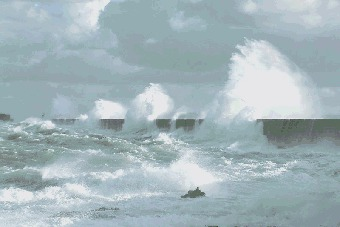
\includegraphics[scale=0.6]{querqueville.jpg}
\end{figure}

\large

\resetcolorseries[24]{verso}
\begin{verso}
\makebox[1em][c]{\lettrine{A}{}} l'horizon, la mer s'\'etend,
Grise et verd\^atre, battue au vent.
\end{verso}

\begin{verso}
Seul sur le sable, la mer m'appelle,
Et je me sens comme infid\`ele.
\end{verso}

\begin{verso}
T'aurais je rat\'e, ma destin\'ee ?
Ouvert \`a toi, mon coeur bless\'e.
\end{verso}

\hfill{26-09-2016}

\pagebreak
\section{\dotfill L'Oiseau Des Mers}

\begin{figure}[h]
\centering
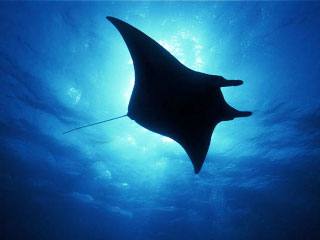
\includegraphics[scale=0.45]{ray.jpg}
\end{figure}

\large

\resetcolorseries[24]{verso}
\begin{verso}
\makebox[1em][c]{\lettrine{T}{}}el un oiseau qui glisse dans l'air,
Mais tes courants sont ceux des mers.
\end{verso}

\begin{verso}
Qu'est ce qui l\`a haut t'a fait plong\'e,
Pour ne jamais y retourner ?
\end{verso}

\begin{verso}
D'un battement d'ailes tu continues,
Vers le grand bleu, vers l'inconnu.
\end{verso}

\hfill{27-09-2016}

\pagebreak
\section{\dotfill Naufrage}

\begin{figure}[h]
\centering
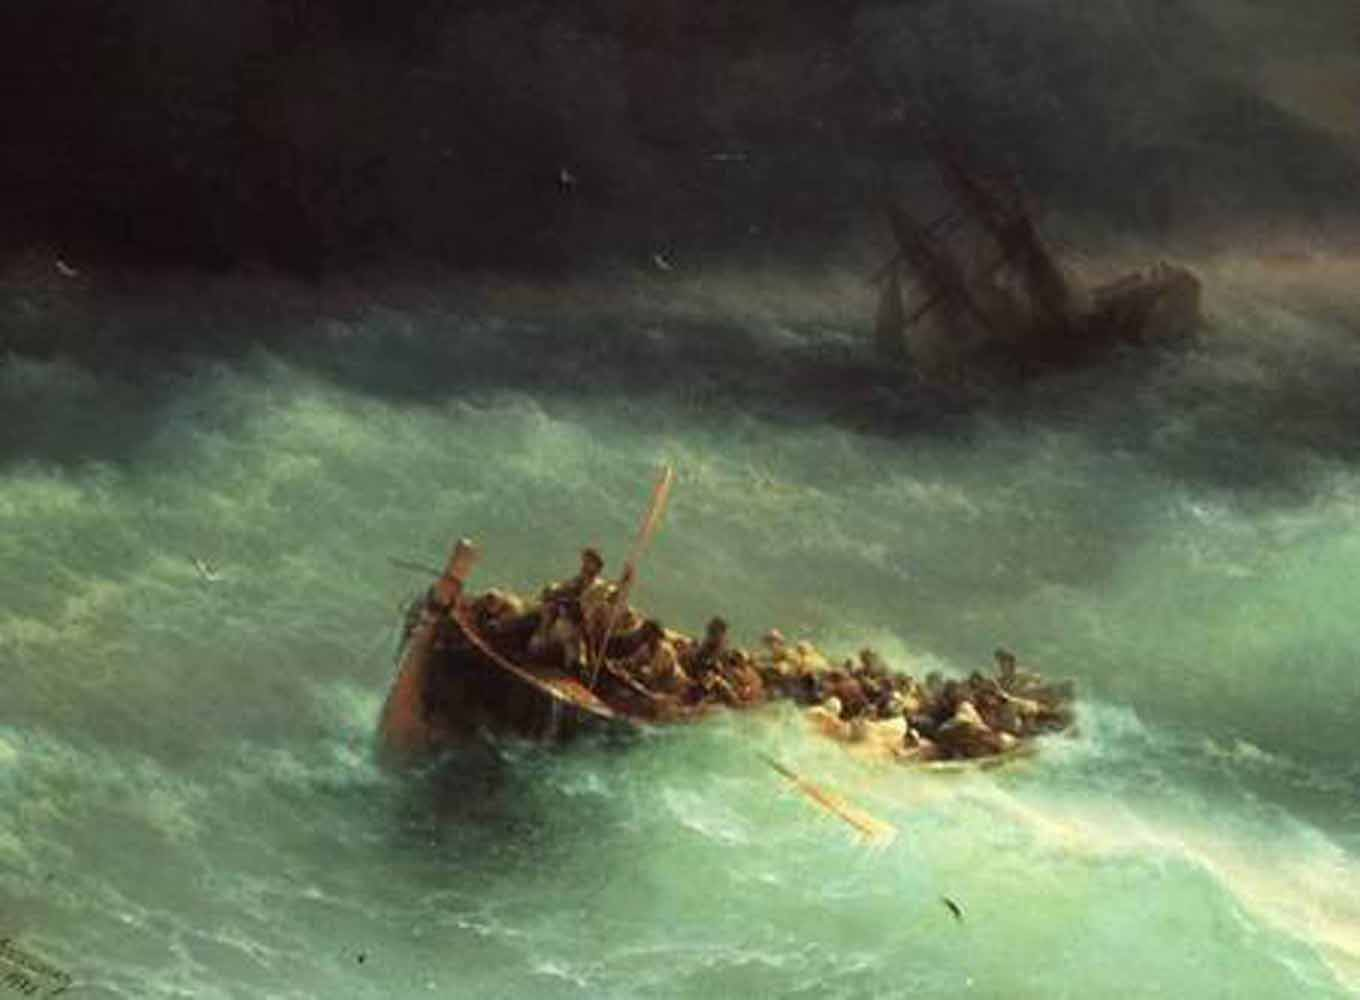
\includegraphics[scale=1]{naufrage.jpg}
\end{figure}

\large

\resetcolorseries[24]{verso}
\begin{verso}
\makebox[1em][c]{\lettrine{T}{}}rop \`a babord,
Trop vers le Nord,
Trop loin du port,
Trop pr\^et des morts.
\end{verso}

\hfill{27-09-2016}


\pagebreak
\section{\dotfill Synchrotron Light}
\large

\begin{figure}[h]
\centering
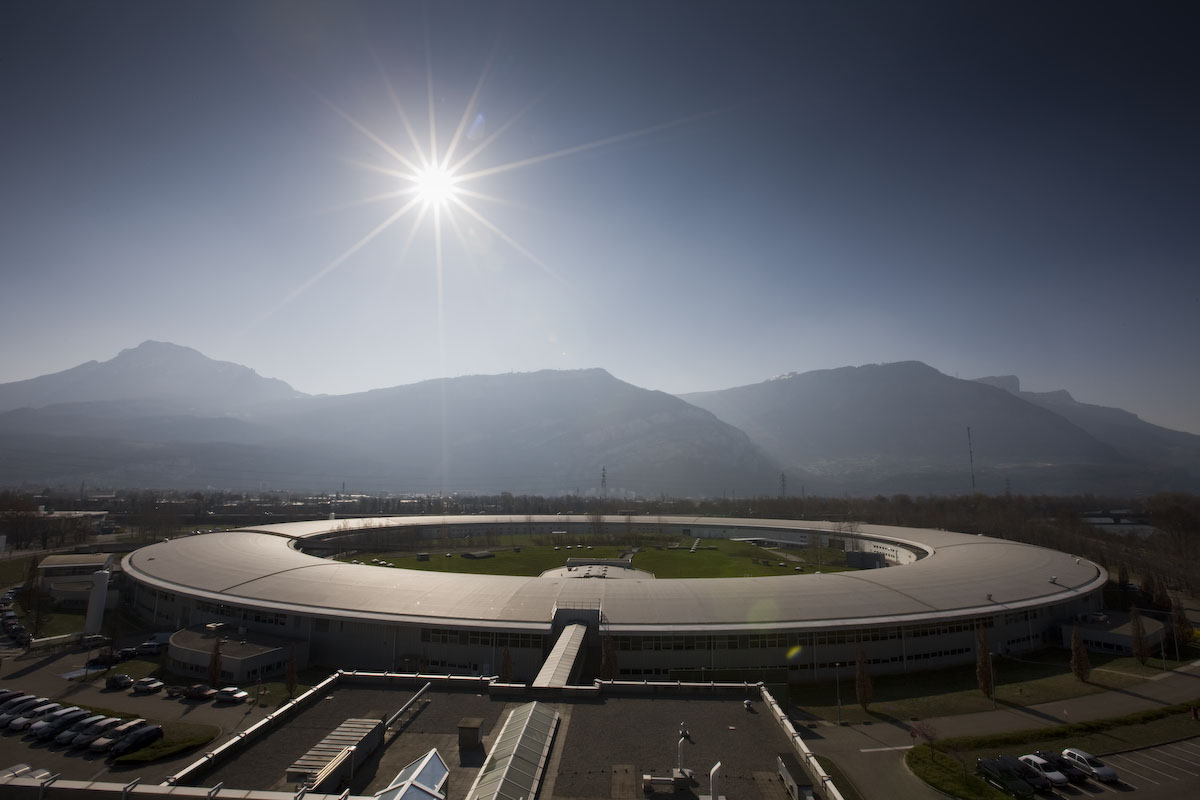
\includegraphics[scale=0.12]{esrf.jpg}
\end{figure}

\resetcolorseries[24]{verso}
\begin{verso}
\makebox[1em][c]{\lettrine{W}{}}ith high voltage the electrons,
Escape as balls from the canons.
\end{verso}

\begin{verso}
They are then accelerated,
Approaching even Light in speed.
\end{verso}

\begin{verso}
Magnetic fields make them deviate,
Loose energy, and radiate.
\end{verso}

\begin{verso}
In the beamlines through slits and glass,
Colors are tuned as the rays pass.
\end{verso}

\begin{verso}
By this process you Giant Rings,
Reveal to us the tiniest things.
\end{verso}

\hfill{29-09-2016}


\pagebreak
\section{\dotfill Papy}
\large

\resetcolorseries[24]{verso}
\begin{verso}
\makebox[1em][c]{\lettrine{P}{}}ortbail durant l'\'et\'e, un gamin et un vieux,
Laissaient trainer leur ligne dans une barque bleue.
\end{verso}

\begin{verso}
Conseils, remarques, astuces, le petit \'ecoutait,
Au large des c\^otes Normandes l'amour des mers naissait.
\end{verso}

\begin{verso}
Il parait loin ce temps, le gamin a grandi,
Mais toujours dans le coeur une place pour son papy.
\end{verso}

\hfill{01-10-2016}


\pagebreak
\section{\dotfill The Submarine}

\begin{figure}[h]
\centering
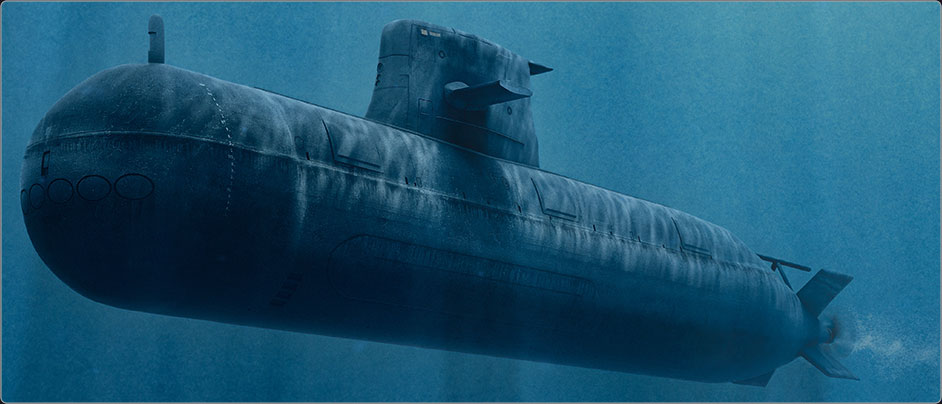
\includegraphics[scale=0.2]{submarine.jpg}
\end{figure}

\large

\resetcolorseries[24]{verso}
\begin{verso}
\makebox[1em][c]{\lettrine{L}{}}urking still in the deep sea night,
It lays silent, ready to fight.
\end{verso}

\begin{verso}
Weeks ago they sank in darkness,
Weeks again 'til they resurface,
\end{verso}

\begin{verso}
They must be strong, the hundred men,
'Cause it\'s a place for the insane.
\end{verso}

\begin{verso}
Heading the crew, the commander,
A word from him, rains the fire.
\end{verso}

\begin{verso}
So here it stands, deadly weapon,
Ready to unleash destruction.
\end{verso}


\hfill{06-10-2016}



\end{document}
